\chapter{Ripple Phase}
When the temperature is reduced from the fluid phase, 
the ripple phase is observed in bilayers consisting of fully saturated lipids.
This chapter discusses X-ray scattering experiments on the ripple phase 
formed by dimyristolphosphatydylcholine (DMPC) bilayers. 

\section{Introduction}
The ripple phase is the greatest thermodynamic phase of lipid bilayers.
This phase was originally found by Tardiue et al. in some lipid bilayers.
What did they find? Further work on the ripple? 

The structure of the ripple phase bilayers can be divided into two categories:
1) the average electron density profile that characterizes how each bilayer
is packed within a stack of lipid bilayers and 2) lateral lipid structure
that characterizes how lipid chains are packed.

Extensive work was done by Wack and Webb (1989). The X-ray form factor
for DMPC was analyzed by Sun et al. Sengupta et al studied the 
temperature dependence of DMPC and other lipids.

Hatchel (1991) did wide angle scattering (transmission) for DPPC.
Rughnathan and Katsaras did near grazing angle WAXS on DMPC.
Sengupta et al. suggested lipid chain packing in 2003 based on 
average bilayer electron density (ED) profile calculated from low angle
X-ray scattering. de Vrie et al suggested interdigitated chain in the
minor side based on molecular dynamics (MD) simulations.

Many theoretical work have been done to understand the origin of
the ripple phase. Some work include Lubensky and Macintosh, ...

These theories predict chain packing in both major
and minor sides. It is obviously important to determine the packing
in order to validate or invalidate those theories. However, this information
is not completely known. WAXS is a direct probe of the chain packing.
It is difficult because scattering is rather weak compared to gel phase. 

Here, we report DMPC average structure calculated from
low angle X-ray scattering data collected at a synchrotron.
Careful analysis allowed us to derive a high resolution ED profile.
The profile suggests WHAT? 

We also report wide
angle X-ray scattering, and suggest chain packing based on both LAXS and WAXS.
Highly brilliant synchrotron X-ray allows high resolution study on 
weak, possibly diffuse scattering.  We determined that the peak is off the 
equator and tilted from the virtical $q_z$ axis.

\section{Materials and Methods}
High resolution was achieved by the use of Germanium monochromator, 0.01\% 
energy dispersion. Low resolution data were taken with multilayer 
monochromator with 1\% energy dispersion.

To achieve small mosaic spread, samples were annealed at 60 \textcelsius for
at least 6 hours right before the experiment. Silicon wafers were cleaned
just before use. 2:1 methanol: chloroform was used to dissolve DMPC.
Sample were rocked continuously during solvent evaporation and dried further
inside a glove box. Samples were then dried under a hood for 24 hours 
and in a vaccume chamber for 2 hours. Samples were stored in a refrigerator.

A thin piece of molybdenum was used to attenuate the beam. The attenuation length
$\mu$ of X-ray in Mo is 6.433 $\mu$m for 8 keV and 13.74 $\mu$m for 10.55 keV 
\cite{ref:cxro}.
For a nominal 25 $\mu$m thick Mo attenuator, $\mu=13.74$ gives the attenuation factor 
of $[\exp(-25/13.74)]^{-1} = 6.2$. The exact attenuation factor was determined
by taking images with and without the attenuator and calculating a factor
that needed to be multiplied for the images to match with each other.

Low angle scattering was done with low resolution setup.

25 $\mu$m silicon wafer was used to deposite our sample. This wafer absorbs
only 20\% of the X-ray beam at 10.5 keV (Check this). This weak absorption
allows transmission scattering. Trasmission experiment was done with
low resolution setup.

Near grazing incident wide angle X-ray scattering experiment was done 
with both high and low resolution setups.
To minimize geometric broadening in grazing angle experiment, the sample
was trimmed to either 1 or 2 mm. 

\subsection{Sample Preparation}
DMPC was purchased from Avanti Polar Lipids and used without further purification.
Oriented thin film was deposited following the rock and roll procedure.  
In previous synchtrotron experiments, the samples were created and annealed 
more than a week in advance and stored in a refrigerator. The orientation
quality of these samples were found to be worse than the quality soon after
the samples were annealed. Therefore, to ensure the best sample quality, the 
sample was annealed for approximately 12 hours just before the X-ray experiment.
Figure X compares a sample scattering in 2011 and 2013 synchrotron runs. 
Because of substantial degree of mosaic spread in the 2011 sample, many peaks
overlapped, rendering the accurate measurement of integrated intensity difficult.
Figure XX shows a picture of the annealing chamber. To achieve gentle but
efficient hydration of a sample, filter papers were installed to cover the 
sample. For successful annealing, it must be emphasized that the annealing 
chamber equilibrates in the over prior to putting the samples in the chamber.
When the sample was put in the chamber with its water at room temperature and
then the system was placed inside the oven, warm vapor condensed on the cooler
sample, causing so called flooding of oriented sample. A small drop of water
on the oriented film was deterimental for the orientation because the bilayers
tend to peel off, resulting in entropy-driven formation of unoriented vesicles 
in the water subphase. 

The sample for grazing incident wide angle study was prepared in the same way 
as for low angle study. In order to minimize the geometric broadening, the 
sample was further trimmed down to 1 mm in width.

The sample for transmission study was deposited on a thin, 35 micron, silicon
wafer. Because the wafer was very fragile, attaching the sample to a sticky 
thing was impossible. Instead, the sample was attached to a plastic cap of 
a small vial with a small amount of heat sink compound at a conrner of the 
wafer. The wafer was stable enough for rocking. The sample deposited on a 
glass cover slip (70 microns) was prepared similarly.  

\subsection{Low Angle X-ray Scattering Experiment}
The same setup as described in Tat chapter was used for low angle diffraction
experiment. In order to achieve a D-spacing comparable to that of Wack and Webb
($D \approx 57.9$ \AA), the current to the Peltier was reversed, which heats the 
Peltier surface the sample was situated on. 

The integrated intensity of each peak was obtained by putting a box around a
peak and summing up the intensity in those pixels that fall inside the box.
The background scattering was estimated by measuring the intensity in pixels
near the peak but not containing any peak tail. The choice of box side was 
made according to the width of each peak. Because of mosaic spread in the sameple,
peaks were wider for higher orders. Accordingly, the box was made wider for higher
orders. The box size was chosen so that approximately 90\% of the peak intensity
was counted toward the integrated intensity.

A few peaks in the ripple phase
were very strong, leading to saturation of CCD pixels. A nominally 25 micron 
molybdinum attenuator was inserted in the upstream to reduce the intensity
of the X-ray beam and one second exposure was collected. The integrated intensity 
of the most strong, (1,0) peak was measured from this short exposure. To
measure the actual attenuation factor, a one second exposure without the 
attenuator was also taken. Comparison of these two images yielded an 
attenuation factor of 7.8. The intensity of (2,0) and (2,-1) peaks were also
measured in this one second exposure with an attenuator. All the other peaks
were observed without saturation in 60 second exposure. To properly scale the 
strong orders, (1,0) peak intensity was multipied by 7.8 x 60 and (2,0) and
(2,-1) were multiplied by 60. 

The integrated intensity, peak position in pixel, the size of box, and estimated
background for all the peaks are shown in Appendix.

\subsection{Near Grazing Incident Wide Angle X-ray Scattering Experiment}
Instead of multilayer monochromator with 1\% energy dispersion, 
silicon monochromator with $\Delta E/E$ of 0.001\% was used to achieve
a higher resolution than that for the low angle X-ray scattering experiment.  

\subsection{Transmission Wide Angle X-ray Scattering Experiment}
The axis of rotation does not coincide with the
plane of the sample, so that the sample-to-detector distance is not fixed
for different motor angle. The sample-to-detector distance was estimated
from the setup geometry. We used 35 $\mu$m thin Si wafer, which absorbs
x-ray by only 10\%. 

\section{Some Theories}
\subsection{Lattice Structure}
It has been shown from X-ray studies (ref) that ripples in in different bilayers
are registered to form a two-dimensional oblique lattice as shown by the unit 
cell in Fig. X. 
The unit cell vectors in the ripple phase can be expressed as 
\begin{equation}
  \mathbf{a} = \frac{D}{\tan\gamma}\xhat + D\zhat
\end{equation}
and
\begin{equation}
  \mathbf{b} = \lambda_r\xhat.
\end{equation}
The corresponding reciprocal lattice unit cell vectors are
\begin{equation}
  \mathbf{A} = \frac{2\pi}{D}\zhat
\end{equation}
and
\begin{equation}
  \mathbf{B} = \frac{2\pi}{\lambda_r}\xhat - \frac{2\pi}{\lambda_r\tan\gamma}\zhat.
\end{equation}
The reciprocal lattice vector, $\mathbf{q}_{hk}$ for the Bragg peak with 
Miller indices $(h,k)$ is 
\begin{equation}
  \mathbf{q}_{hk}=h\mathbf{A}+k\mathbf{B},
\end{equation}
so its Cartesian components are
\begin{align}
  & q_{k}^x \equiv q_{hk}^x = \frac{2\pi k}{\lambda_r} \\
  & q_{hk}^y = 0 \\
  & \qz{hk} = \frac{2\pi h}{D} - \frac{2\pi k}{\lambda_r\tan\gamma}.
\end{align}


%%%%%%%%%%%%%%%%%%%%%%%%%%%%%%%%%%%%%%%%%%%%%%%%%%%%%%%%%%%%%%%%%%%%%%%%%%%%%%%
\subsection{Sample $q$-space}
The incoming and outgoing wavevectors of the x-ray beam in Fig. XXX 
are given by
\begin{equation}
  \kin = \frac{2\pi}{\lambda} \yhat, \quad
  \kout = 
    \frac{2\pi}{\lambda} \left( 
      \sin 2\theta \cos\phi \, \xhat
      + \cos 2\theta \, \yhat
      + \sin 2\theta \sin\phi \, \zhat 
    \right),
  %\label{eq:kinkout}
\end{equation}
where $\lambda$ is the wavelength of x-ray, $2\theta$ is the total scattering
angle, and $\phi$ is the angle measured from the equator on the detector. 
The scattering vector (also called
momentum transfer vector) is
the difference between $\kin$ and $\kout$,
\begin{align}
  \mathbf{q} &= \kout - \kin \nonumber \\
             &= q \left( 
                  \cos\theta\cos\phi \, \xhat - \sin\theta \, \yhat
                  + \cos\theta\sin\phi \, \zhat
                \right),
  \label{eq:q_vector}
\end{align}
where $q=4\pi\sin\theta/\lambda$ is the magnitude of the scattering vector. 
When the sample is rotated by $\omega$ about the lab x-axis in the clockwise 
direction as shown in Fig. XXX, the sample $q$-space also rotates and 
are given by  
\begin{equation}
  \mathbf{\hat{e}_x} = \xhat, \quad
  \mathbf{\hat{e}_y} = \cos\omega\,\yhat + \sin\omega\,\zhat, \quad
  \mathbf{\hat{e}_z} = -\sin\omega\,\yhat + \cos\omega\,\zhat.
  \label{eq:smp_coord}
\end{equation}
From Eq.~(\ref{eq:q_vector}) and (\ref{eq:smp_coord}), we find the sample
$q$-space to be
\begin{align}
  q_x &= \mathbf{q}\cdot\mathbf{\hat{e}_x} 
       = q\cos\theta\cos\phi, 
       \nonumber\\
  q_y &= \mathbf{q}\cdot\mathbf{\hat{e}_y} 
       = q\left(-\sin\theta\cos\omega + \cos\theta\sin\phi\sin\omega\right), 
       \nonumber\\
  q_z &= \mathbf{q}\cdot\mathbf{\hat{e}_z} 
       = q\left(\sin\theta\sin\omega + \cos\theta\sin\phi\cos\omega\right).
       \label{eq:qxqyqz}
\end{align}
The position, $(X,Z)$, of a CCD pixel is measured with respect to the beam 
and given by
\begin{equation}
  X = S \tan 2\theta \cos\phi, \quad Z = S \tan 2\theta \sin\phi,
  \label{eq:XZ}
\end{equation} 
where $S$ is the distance between the sample and detector.
From a model for the electron density of a lipid bilayer, one calculates
a X-ray scattering intensity pattern, $I(\mathbf{q})$. Then, Eq.~(\ref{eq:qxqyqz})
and (\ref{eq:XZ}) relate $I(\mathbf{q})$ to the experimentally measured
intensity pattern, $I(X,Z)$. It is important to remember that a given pixel
position, $(X,Z)$, corresponds to a triplet $(q_x, q_y, q_z)$. Fully exploring 
the sample $q$-space requires changing $\omega$ for a fixed wavelength, which was
achieved by continuously rotating the sample with a motor. In the ripple phase, 
because our sample has in-plane rotational symmetry,
the ripple side peaks make up Bragg rings while the main peaks are still 
delta function like (see Fig. X) in $q$-space. In order for the main peak to be
observed, $\omega$ must be equal to $\theta_\mathrm{B}$, but the side peaks
are observed at any $\omega$. Those side peaks get slightly smeared due to 
integration over $q_y$.

For low angle x-ray scattering (LAXS), it is convenient to linearize the above
equations in terms of $\theta$ and $\omega$. In the small angle approximation, 
$\sin\phi \approx Z/(2S\theta)$ and $\cos\phi \approx X/(2S\theta)$, and
\begin{align}
  q_x &\approx \frac{4\pi\theta\cos\phi}{\lambda} \approx kX/S \nonumber\\
  q_y &\approx q_z\omega -\frac{4\pi\theta^2}{\lambda} \approx q_z\omega - \frac{\lambda q_z^2}{4\pi}\nonumber\\
  q_z &\approx \frac{4\pi\theta\sin\phi}{\lambda} \approx kZ/S,
  \label{eq:qxqyqz_small}
\end{align}
with $k=2\pi/\lambda$. For wide angle X-ray scattering, the exact relations given
by Eq.~(\ref{eq:qxqyqz}) are necessary. Especially in the transmission experiment,
where $\omega$ is large, an observed X-ray pattern appears nontrivial and becomes
almost impossible to analyze without the use of Eq.~(\ref{eq:qxqyqz}).


%%%%%%%%%%%%%%%%%%%%%%%%%%%%%%%%%%%%%%%%%%%%%%%%%%%%%%%%%%%%%%%%%%%%%%%%%%%%%%%
\subsection{Geometric (Lorentz) Correction}\label{sec:Lorentz_correction}
Our sample has in-plane rotational symmetry. This means that the sample 
consists of many domains with differing ripple directions, all domains
being parallel to the substrate.  
In sample $q$-space, then, ripple side peaks become rings while main peaks are
still points (see Fig. X). For an arbitrary incident angle, main peaks are not observed
while side peaks are observed. 
In order to capture both main and side peaks in one X-ray exposure, 
the sample was continuously rotated. As a result of this rotation, 
main peaks become arcs that subtend an angle $2\theta_{h0}$,
as shown in Fig.~\ref{fig:ewald_main}, with its length
equal to $2\theta_{h0}\qz{h0}$.  
%------------------------------------------------------------------------------
\begin{figure}[htbp]
  \centering
  \includegraphics[scale=1]{figures/ripple/ewald_main2}
  \caption{caption goes here}
  \label{fig:ewald_main}
\end{figure}
%------------------------------------------------------------------------------
The detector records the cross sections of these arcs with the 
Ewald sphere, so the total scattering power is the product of the observed intensity,
$\Io{hk}$ with the arc length, that is, 
\begin{equation}
  I = 2\theta_{h0}\qz{h0} \Io{h0}. \label{eq:main_ewald}
\end{equation}

Because the sample has in-plane rotational symmetry, side peaks are represented as
rings whose radius is $\qr{hk}$. For a fixed incident
angle, all the rings are intersected by the Ewald sphere. Because only the domains
with the right ripple direction can satisfy the Bragg's condition at a given fixed
angle, the scattering power of this small cross section is reduced by 
a factor of $2\pi \qr{k}$ compared to main peaks. During 
an X-ray exposure, the rings cross the Ewald sphere
at all incident angles. Then, the total scattering power is given by
\begin{equation}
  I=2\pi \qr{k} \Io{k}. \label{eq:side_ewald}
\end{equation}
Inverting Eq.~(\ref{eq:main_ewald}) and (\ref{eq:side_ewald}) 
and realizing that the intensity is the form factor
squared, we can calculate the observed intensity, $\Io{}$, 
from a model for an electron density in the ripple phase.
%------------------------------------------------------------------------------
\begin{figure}[htbp]
  \centering
  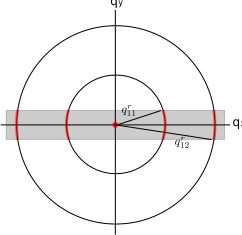
\includegraphics[scale=1]{figures/ripple/ewald_side_h1_ver1}
  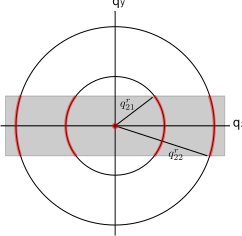
\includegraphics[scale=1]{figures/ripple/ewald_side_h2_ver1}
  \caption{$q$-space representations of Bragg peaks and Bragg rings 
  for $h=1$ and $k$ = 0, 1, and 2 in $\qz{hk}$ planes.
  The shaded rectangles show cross sections of the rotating Ewald sphere along
  $\qz{hk}$ plane. The intersection between the Ewald sphere and 
  a Bragg peak/ring is indicated in red. 
  The observed intensity for the $k\neq 0$ orders is proportional to
  the fraction of the length of red arcs in the circumference. This 
  fraction is equal to one for a $k=0$ order.
  Because the orders are not in the same $q_z$ plane, the range of $q_y$ 
  integration indicated by the height of the rectangle is different for different
  orders. The magnitude of curvature of arcs is exaggerated.}
  \label{fig:ewald_side_h1}
\end{figure}
%------------------------------------------------------------------------------

Mathematically, the rotation is  
equivalent to an integration over $\omega$. In low angle X-ray scattering, 
$q_z$ is constant at a given pixel as $\omega$ is changed, which can be seen from 
Eq.~(\ref{eq:qxqyqz_small}). $\omega$ dependence appears only through $q_y$, 
so rotating the sample is realized by integrating over $q_y$. 
To derive the integration limits, let us consider two cases: (a) When $\omega \leq 0$,
the incoming X-ray beam is blocked by the back of the substrate. This sets 
the lower limit to 0. (b) When $\omega \geq 2\theta$, the substrate blocks 
the outgoing X-ray. Within the small angle approximation, then, $\omega_{\text{max}}$
is $2\times \lambda q_z/(4\pi)$ for scattering with $q_z$. 
Thus, the integration limits 
for $q_y$ integration are $[-\lambda q_z^2/(4\pi), \lambda q_z^2/(4\pi)]$.
We also need to integrate over $X$ and $Z$ to obtain integrated intensity. 
These lead to the observed intensity
written as,
\begin{align}
  \Io{hk} 
    &\propto \int dX \int dZ \int d\omega |F_{hk}|^2 S_{hk}(\mathbf{q}) \nonumber \\
    &\propto |F_{hk}|^2 \int dq_x \int dq_z 
             \int_{-\frac{\lambda q_z^2}{4\pi}}^{\frac{\lambda q_z^2}{4\pi}} 
             \frac{dq_y}{q_z} 
             S_{hk}(\mathbf{q}),
\end{align}
where $1/q_z$ factor in $q_y$ integration is the Lorentz polarization factor
in the small angle approximation. 

For a crystalline sample with the in-plane rotational symmetry, the
structure factor is  
\begin{equation}
  S_{hk}(\mathbf{q}) = S_{hk}(q_r,q_z) 
  = \frac{1}{2\pi q_r}\delta(q_r-q_{r,k})\delta(q_z-q_{z,hk}),
\end{equation} 
where $q_{r,k}=2\pi |k|/\lambda_r$. Thus, the scattering pattern in the 
ripple phase is a 
collection of Bragg ``rings'' centered at the meridian and the 
Bragg peaks that are called the main peaks.  

The observed, integrated intensity of $hk$ peak is proportional to
\begin{equation}
  I_{\mathrm{o},hk} 
    \propto \frac{\lvert F_{hk} \rvert^2}{q_{z,hk}} \int\mathop{dq_x} 
            \int_{-q_{y0}}^{q_{y0}}
            \mathop{dq_y} \frac{\delta(q_r-q_{r,k})}{2\pi q_r},
\end{equation}
where $q_{y0} = \lambda q_{z,hk}^2/(4\pi)$.
For side peaks ($k \neq 0$), we have 
\begin{align}
  \int\mathop{dq_x} \int_{-q_{y0}}^{q_{y0}}\mathop{dq_y} \frac{\delta(q_r-q_{r,k})}{2\pi q_r}
  &\approx \int_{-\frac{q_{y0}}{q_{r,k}}}^{\frac{q_{y0}}{q_{r,k}}} \mathop{d\phi} 
          \int \mathop{dq_r} q_r\frac{\delta(q_r-q_{r,k})}{2\pi q_r} \nonumber\\
 &= \frac{q_{y0}}{\pi q_{r,k}}. \label{eq:side_integrand}
\end{align}
For main peaks ($k=0$), we have 
\begin{align}
  \int\mathop{dq_x} \int_{-q_{y0}}^{q_{y0}}\mathop{dq_y} \frac{\delta(q_r-q_{r,k})}{2\pi q_r}
  &= \int_0^{2\pi}\mathop{d\phi} \int\mathop{dq_r} q_r\frac{\delta(q_r-q_{r,k})}{2\pi q_r} \nonumber\\
  &= 1 \label{eq:main_integrand}
\end{align}
Using Eq.~(\ref{eq:side_integrand}) and (\ref{eq:main_integrand}), 
we write the observed integrated intensity as
\begin{align}
  I_{\mathrm{o},h0} &\propto \frac{|F_{h0}|^2}{q_{z,h0}} \label{eq:main}\\
  I_{\mathrm{o},hk} &\propto \frac{|F_{hk}|^2}{q_{z,hk}} \frac{q_{y0}}{\pi q_{r,k}}
    = |F_{hk}|^2 \frac{\lambda q_{z,hk}}{2\pi}\frac{1}{2\pi q_{r,k}}
    = |F_{hk}|^2 \frac{2\theta_{hk}}{2\pi q_{r,k}}, \label{eq:side}
\end{align}
where $2\theta_{hk} = \lambda q_{z,hk}/(2\pi)$ is the incident angle at which 
the outgoing X-ray for the peak $(hk)$ is blocked by the substrate.
Eq.~(\ref{eq:main}) and (\ref{eq:side}) relate the form factor calculated from
a model to the experimentally observed intensity, and are 
equivalent to Eq.~(\ref{eq:main_ewald}) and (\ref{eq:side_ewald}), 
which were derived by using the Ewald sphere. 

In nonlinear least-squares fitting procedure, 
we fitted the observed integrated intensity to
the calculated intensity from a bilayer model using these geometrical corrections. 
This is because we can determine experimental uncertainties
on observed intensity rather than the geometrically corrected form factors. 
We avoid propagating the uncertainties by fitting a model to observed intensity. 

%%%%%%%%%%%%%%%%%%%%%%%%%%%%%%%%%%%%%%%%%%%%%%%%%%%%%%%%%%%%%%%%%%%%%%%%%%%%%%%
\subsection{Absorption Correction for LAXS}
In this section, we derive the absorption correction for the thin film
sample. The calculation involves an explicit integration over the incident angle, 
$\omega$, which is necessiated by the sample rotation during an x-ray exposure. 
The procedure is to write down an absorption factor, $A(\omega,\theta)$, for a 
given scattering angle at a given incident angle, and
then integrate over $\omega$. We ignore $q_x$ dependence because the X-ray
path inside the sample is nearly within the $y$-$z$ plane for low angle
scattering. The correction for wide angle scattering is described in a later
section.

Assume that all the X-rays enter the sample from the top surface. The total scattering
angle is given by $2\theta$ (see Fig.~\ref{fig:absorption_LAXS}).
%------------------------------------------------------------------------------
\begin{figure}[htbp]
  \centering
  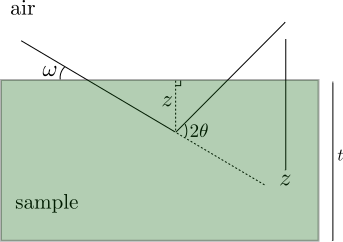
\includegraphics[scale=1]{figures/ripple/absorption_LAXS}
  \caption{The path of X-rays within the sample. The incident angle is 
  $\omega$ and the total scattering angle is $2\theta$. An X-ray with a
  penetration depth of $z$ is shown. The total thickness of the sample
  is $t$.}
  \label{fig:absorption_LAXS}
\end{figure}
%------------------------------------------------------------------------------
Let $z$-axis point downward. At the top surface
(air-sample interface), $z=0$. For X-rays that travel to $z$ and then scatter, the
total path length within the sample is 
\begin{equation}
  L_\textrm{tot}(z,\omega,\theta) 
  = \frac{z}{\sin\omega}+\frac{z}{\sin(2\theta-\omega)} 
  = zg(\omega,\theta),
\end{equation}
where $g(\omega,\theta)=(\sin\omega)^{-1}+\pars{\sin\pars{2\theta-\omega}}^{-1}$.
For each ray, the intensity is attenuated by the sample absorption. 
If non-attenuated 
intensity is equal to $I_0$, then the attenuated intensity is
\begin{equation}
  I(z,\omega,\theta) = I_0\exp\left(-\frac{L_\textrm{tot}}{\mu}\right),
  \label{eq:ray}
\end{equation}
where $\mu$ is the absorption length of an X-ray. $\mu$ is 111 for 10.5 keV
and 222 for 8 keV \cite{ref:cxro}.
The observed intensity of scattering from a sample fixed at an angle $\omega$ 
is equal to the integration
of Eq.~(\ref{eq:ray}) over the whole sample and given by
\begin{align}
  I_{\textrm{obs}}(\omega,\theta) 
    &= \int_0^t \dz I(z,\omega,\theta)
     = I_0\int_0^t\dz \exp\left(-\frac{g(\omega,\theta)}{\mu}z\right) \nonumber \\
    &= I_0\mu \frac{1-\exp\left(-\frac{t}{\mu}g(\omega,\theta)\right)}{g(\omega,\theta)}.
    \label{eq:I_obs1}
\end{align}
Defining the absorption factor at a fixed angle to be $A(\omega,\theta)$, 
the observed intensity can be written as
\begin{equation}
I_{\textrm{obs}}(\omega,\theta)=A(\omega,\theta)tI_0,
\label{eq:I_obs2}
\end{equation}
where $tI_0$ is the intensity we would observe for non-absorbed X-rays.
Equating Eq.~(\ref{eq:I_obs1}) and (\ref{eq:I_obs2}), we get
\begin{equation}
  A(\omega,\theta) = \frac{\mu}{t} 
                     \frac{1-\exp\left(-\frac{t}{\mu}g(\omega,\theta)\right)}{g(\omega,\theta)}.
\end{equation}
The total observed intensity from a sample that is being rotated during 
an exposure is simply
\begin{equation}
  I_{\textrm{total}}(\theta) 
  = \int_0^{2\theta}\textrm{d}\omega I_{\textrm{obs}}(\omega,\theta).
\end{equation}
The upper integration limit is equal to $2\theta$ because the substrate
completely blocks the scattered X-rays above this angle as discussed in 
section \ref{sec:Lorentz_correction}.

Because the total non-attenuated intensity is given by $t\omega I_0$,


so that the total absorption factor is equal to
\begin{equation}
  A(\theta) = \frac{\mu}{2\theta t} \int_0^{2\theta}d\omega 
      \frac{1-\exp\left(-\frac{t}{\mu}g(\omega)\right)}{g(\omega)}.
\end{equation}
If $\mu$ is taken to infinity (no absorption), $A$ goes to 1 as expected. 
Here, it is important to note that $1/2\theta$ factor in the above equation
is normally called Lorentz polarization factor, which
is usually approximated as $1/q_z$ for LAXS analysis. Since the SDP
program applies this correction factor in addition to the absorption
correction, we remove this factor in the formula for $A_c$. Therefore,
the final result for the total absorption correction is 
\begin{equation}
  A_c(\theta) 
    = \frac{1}{2\theta A(\theta)} \nonumber \\
    = \frac{t}{\mu} 
       \left[ 
         \int_0^{2\theta}d\omega 
         \frac{1-\exp\left(-\frac{t}{\mu}g(\omega)\right)}{g(\omega)}
       \right]^{-1}
\end{equation}
with $g(\omega)=1/\sin\omega+1/\sin(2\theta-\omega)$.

%%%%%%%%%%%%%%%%%%%%%%%%%%%%%%%%%%%%%%%%%%%%%%%%%%%%%%%%%%%%%%%%%%%%%%%%%%%%%%%
\subsection{Absorption Correction for WAXS}

%%%%%%%%%%%%%%%%%%%%%%%%%%%%%%%%%%%%%%%%%%%%%%%%%%%%%%%%%%%%%%%%%%%%%%%%%%%%%%%
\section{Model}
\subsection{Contour Part of the Form Factor}
As in ref, we take the ripple profile to have a sawtooth-like profile. Its
amplitude is  $A/2$ and the projection of the major arm on the 
ripple direction is $x_0$ as shown in Fig. X. Then, we write the ripple 
profile as
\begin{equation}
  u(x) = \left\{
    \begin{array}{ccc}
    -\frac{A}{\lambda_r-x_0}\left(x+\frac{\lambda_r}{2}\right) 
      & \text{for} 
      & -\frac{\lambda_r}{2} \leq x < -\frac{x_0}{2}, \\
    \frac{A}{x_0}x 
      & \text{for} 
      & -\frac{x_0}{2} \leq x \leq \frac{x_0}{2}, \\
    -\frac{A}{\lambda_r-x_0} \left(x-\frac{\lambda_r}{2}\right)
      & \text{for} 
      & \frac{x_0}{2} < x \leq \frac{\lambda_r}{2}.
    \end{array} \right.
\end{equation}
The ripple profile has the inversion symmetry, so that the resulting
form factor is real. $A$ and $x_0$ are fitting parameters that depend 
on the integrated intensity of each peak while $D$ and $\lambda_r$ are
determined from measuring the positions of the Bragg peaks.

In order to allow the electron density along the ripple direction to 
modulate, we include two additional parameters, one to allow for the electron
density across the minor side to be different by a ratio $f_1$ from the 
electron density across the major side and a second parameter $f_2$, which
is multiplied by $\delta$ functions $\delta(x \pm x_0/2)$ to allow for 
a different electron density near the kink between the major and the minor
sides. 


%%%%%%%%%%%%%%%%%%%%%%%%%%%%%%%%%%%%%%%%%%%%%%%%%%%%%%%%%%%%%%%%%%%%%%%%%%%%%%%
\subsection{Transbilayer Part of the Form Factor}
\subsubsection{SDF}
Delta function model is described here.

\subsubsection{2G model}
In the hybrid model, the terminal methyl region of the bilayer is represented
as a Gaussian function \cite{ref:Wiener89}. The headgroups are represented by one 
and two Gaussian
functions in 1G and 2G hybrid model, respectively. The methylene and water 
regions are each treated as a constant. The gap between the two constants is 
represented by a sine function. Then, for half of the bilayer, 
$0 \leq z \leq D/2$, the electron density has the form, 
\begin{equation}
  \rho(z) = \rhog(z) + \rhos(z) + \rhob(z),
\end{equation}
where the Gaussian part is given by 
\begin{equation}
  \rhog(z) = \sum_{i=1}^{1\text{ or }2} \rhoh{i}
             e^{-(z-\zh{i})^2/(2\sigmah{i}^2)} + \rhom e^{-z^2/(2\sigmam^2)},
\end{equation}
the strip part is given by
\begin{equation}
  \rhos(z) = \left\{
    \begin{array}{ccc}
      \rhochtwo & \text{for } & 0 \leq z < \zchtwo, \\
      \rhow   & \text{for } & \zw \leq z \leq D/2,
    \end{array}
  \right.
\end{equation}
and the bridging part is given by
\begin{equation}
  \rhob(z) = \frac{\rhow-\rhochtwo}{2} \cos \bracks{
    \frac{-\pi}{\deltazh}(z-\zw)} + \frac{\rhow+\rhochtwo}{2} \\
  \text{\quad for \quad} \zchtwo < z < \zw.
\end{equation}
with $\deltazh=\zw-\zchtwo$. Here, we assume $\zh{2}>\zh{1}$. 
Table \ref{tb:zchtwozw} shows some of the definitions.
%------------------------------------------------------------
\begin{table}[htb]
  \centering
  \begin{tabular}{c c c}
     & 1G & 2G \\
    $\zchtwo$ & $\zh{1}-\sigmah{1}$ & $\zh{1}-\sigmah{1}$ \\
    $\zw$ & $\zh{1}+\sigmah{1}$ & $\zh{2}+\sigmah{2}$   
  \end{tabular}
  \caption{Definitions of $\zchtwo$ and $\zw$}
  \label{tb:zchtwozw}
\end{table}
%------------------------------------------------------------
The transbilayer profile along $x=-z\tan\psi$ can be obtained by rotating
the coordinates $x$ and $z$ by $\psi$ in the clockwise direction and
reexpressing $\rho(z)$ in terms of the rotated coordinates. This leads
to replaincg $x$ with $x'=x\cos\psi+z\sin\psi$ and
$z$ with $z'=-x\sin\psi+z\cos\psi$. Then, the rotated transbilayer profile is
\begin{equation}
  \rho(x,z) = \delta(x+z\tan\psi)\bracks{\rhog(z') + \rhos(z') + \rhob(z')}.
  \label{eq:rotated_profile}
\end{equation}

Taking the two dimensional Fourier transform of Eq.~(\ref{eq:rotated_profile})
leads to the transbilayer part of the form factor,
\begin{align}
  F_\mathrm{T} 
  &= \int_{-\frac{D}{2}}^{\frac{D}{2}} \int_{-\frac{\lambda_r}{2}}^{\frac{\lambda_r}{2}} 
     \bracks{\rho(x,z)-\rhow} e^{i(q_xx+q_zz)} dxdz \\
  &= F_\mathrm{G} + F_\mathrm{S} + F_\mathrm{B}.
\end{align}
The form factor is calculated in the minus fluid convention, 
where the bilayer electron density
is measured with respect to the electron density of the surrounding solvent.
The expression for $F_\mathrm{T}$ is rather messy and not shown. 
The derivation and full expression can be found in the appendix. Here, 
we note that
the fitting parameters in this model are $\zh{i}$, $\sigmah{i}$, and 
$\Rhm{i}$ for each of the two headgroup Gaussian functions, $\sigmam$ for
the terminal methyl Gaussian, $\Delta R$ for the methylene region, $\psi$ for
the lipid tilt, and an overall scaling factor. The contour part of the 
form factor has four more parameters ($A$, $x_0$, $f_1$, and $f_2$).
In total, the modified 2G hybrid model implements 14 structural parameters.


\section{Results}
\subsection{Data}
Table~\ref{tb:lattice_const} summarizes data we analyzed. 
%------------------------------------------------------------
\begin{table}[htb]
  \centering
  \begin{tabular}{c c c c}
       & $\lambda_r$ & $D$ & $\gamma$ \\
    WW & 141.7 & 57.94 & 98.4\degree \\
    S1 & 145   & 57.8  & 98.2\degree \\
    S2 & ? & ? & ?
  \end{tabular}
  \caption{Lattice constants}
  \label{tb:lattice_const}
\end{table}
%------------------------------------------------------------
As shown, we measured scattering in a almost identical conditions as the
Wack and Webb's. This data allowed us to check our data obtained by using
an oriented sample against an unoriented sample. As discussed earlier, 
these two types of samples give different Lorentz correction. We derived
the Lorentz correction for our oriented sample. Applying the derived correction
to our data and calculating the form factor, we were able to confirm our 
correction. This check is shown in Table.

Figure shows a LAXS pattern from DMPC at 18 \degC. $D=57.9$ \AA. Low
resolution experiment. Up to $h=9$ orders were observed in this
data set. Because of a non-negligible degree of mosaicity in the sample,
strong orders cast their arcs over weaker orders. A care must be 
taken to decompose the intensity at a given pixel to intensity due to
a strong order's arc and to that due to a weak peak. This was achieved
by taking a $q_z$ swath and fitting the intensity to two Gaussian
functions whose widths were determined from the known instrumental 
resolution. Figure shows an example of this operation. Table and
Table show with and without the decomposition operation, respectively. 
For many of the orders observed, errors one would expect from 
neglecting the mosaicity effect were small. For higher orders, however,
this was crucial to obtain the correct integrated intensity.

In order to test the decomposition effect, fits were also performed
for the sum of intensity for orders that overlap. 

First, we fitted the data using only up to $h=3$ orders. What did we get?
How did each model do? Any inconsistency witht
 Sun PNAS?

Next, we fitted every peak we observed. Which model failed?

%%%%%%%%%%%%%%%%%%%%%%%%%%%%%%%%%%%%%%%%%%%%%%%%%%%%%%%%%%%%%%%%%%%%%%%%%%%%%%%
\subsection{Electron Density Profile}
Table X shows the best fit for each model. It shows that the delta function
model fails. Its failure is obviously due to its lack of fine structural 
details. In ref. (SUN), the model marginally worked because only up to
the third orders were available. With the high flux synchrotron X-ray beam,
many more higher orders were observed, whose intensity is dominated by
finer details in the bilayer electron density. The table shows that
1G model also fails. 2G model works, but simple 2G model failed. $k=6$ orders
clearly require the modulation in the electron density along the ripple 
direction. The phase of lower orders tends to be the same throughout
the different models while higher orders vary widely. These are just ideas.
I need to do actual fitting.

\subsection{Near Grazing Incident Wide Angle X-ray Scattering (NGIWAXS)}
Convert the image to $q$-space. Show the two resolved peaks.
Measure the positions of these peaks. Can we confirm  that
the observed weak diffuse scattering is not the mosaic spread, but
true sample scattering? Comment on the widths of the peaks observed.
Possibly make use of both low and high resolution data.
Apply the absorption correction.

\subsection{Transmission WAXS}
Convert the image to $q$-space.
No strong order on the equator. Subtraction of water scattering from the
background image. Compare to NGIWAXS and comment on the absorption effect
in NGIWAXS data.

\section{Discussion}
Comparison with previous unoriented/oriented stuff?

Which theories are consistent/inconsistent with the results of this study?


\section{Conclusion}
Well, the ripple phase is the greatest phase in the lipid bilayers. Our detailed
work lead to deeper insight into the formation of this phase. Future experiments
include the high resolution transmission experiment, where both geometric 
broadening and energy dispersion are minimized. The expected resolution 
is the width of the X-ray beam, which is about 3 pixels. This experiment 
doubles the best resolution achieved in this work. 
Another slightly different high resolution experiment is to use silicon 
crystal analyzer downstread of the sample, which completely remove geoemtric
boradening. The downside of this type of high resolution experiment is that
only one point in q-space is probed at any given exposure, so to get a full
2D map of wide angle scattering is time consuming.  
